\documentclass[12pt,letterpaper]{article}
\usepackage{fullpage}
\usepackage[top=2cm, bottom=4.5cm, left=2.5cm, right=2.5cm]{geometry}
\usepackage{amsmath,amsthm,amsfonts,amssymb,amscd}
\usepackage{lastpage}
\usepackage{enumerate}
\usepackage{fancyhdr}
\usepackage{mathrsfs}
\usepackage{xcolor}
\usepackage{graphicx}
\usepackage{listings}
\usepackage{hyperref}

\hypersetup{%
  colorlinks=true,
  linkcolor=blue,
  linkbordercolor={0 0 1}
}
 
\renewcommand\lstlistingname{Algorithm}
\renewcommand\lstlistlistingname{Algorithms}
\def\lstlistingautorefname{Alg.}

\lstdefinestyle{Python}{
    language     = Python,
    aboveskip    = 3mm,
    belowskip    = 3mm,
    frame        = lines, 
    basicstyle   = \footnotesize\ttfamily,
    keywordstyle = \color{blue},
    stringstyle  = \color{green},
    commentstyle = \color{red}\small\ttfamily
}

\setlength{\parindent}{0.0in}
\setlength{\parskip}{0.05in}


% Edit these as appropriate
\newcommand\course{CSE 3500}
\newcommand\hwnumber{4}                  % <-- homework number
\newcommand\release{10/13/2022}    % <-- release date
\newcommand\due{10/20/2022}        % <-- homework number

\pagestyle{fancyplain}
\headheight 20pt
\lhead{mfm19005}
\chead{\textbf{\Large Homework \hwnumber}}
\rhead{October 17th, 2022}
\lfoot{}
\cfoot{}
\rfoot{\small\thepage}
\headsep 1.5em

\begin{document}

\begin{center}
    \LARGE Suffix Trees, Hashing
\end{center}


\section*{Problem 0 -- Suffix Trees on multiple strings (25\%)}
A suffix tree of $m$ strings $(S_1,S_2,\dots,S_m)$ is a suffix tree built from inserting the strings in order: $S_1\$_1$, $S_2\$_2$, $\dots$, $S_m\$_m$ where $\$_1,\dots,\$_m$ are distinct terminating strings.

\begin{enumerate}
    \item Build the suffix tree for BANDANNA\# and SAVANNAH\$.
    \item Give an algorithm to find the longest common substring of $m$ strings, $S_1,\dots,S_m$ using suffix trees. 
    \item What is your algorithms runtime? Show your work/give an argument.
    \item Using your algorithm, what is the longest common substring of BANDANNA\# and SAVANNAH\$?
\end{enumerate}

\subsection*{Part 1}

\begin{figure}[!htb]
    \centering
    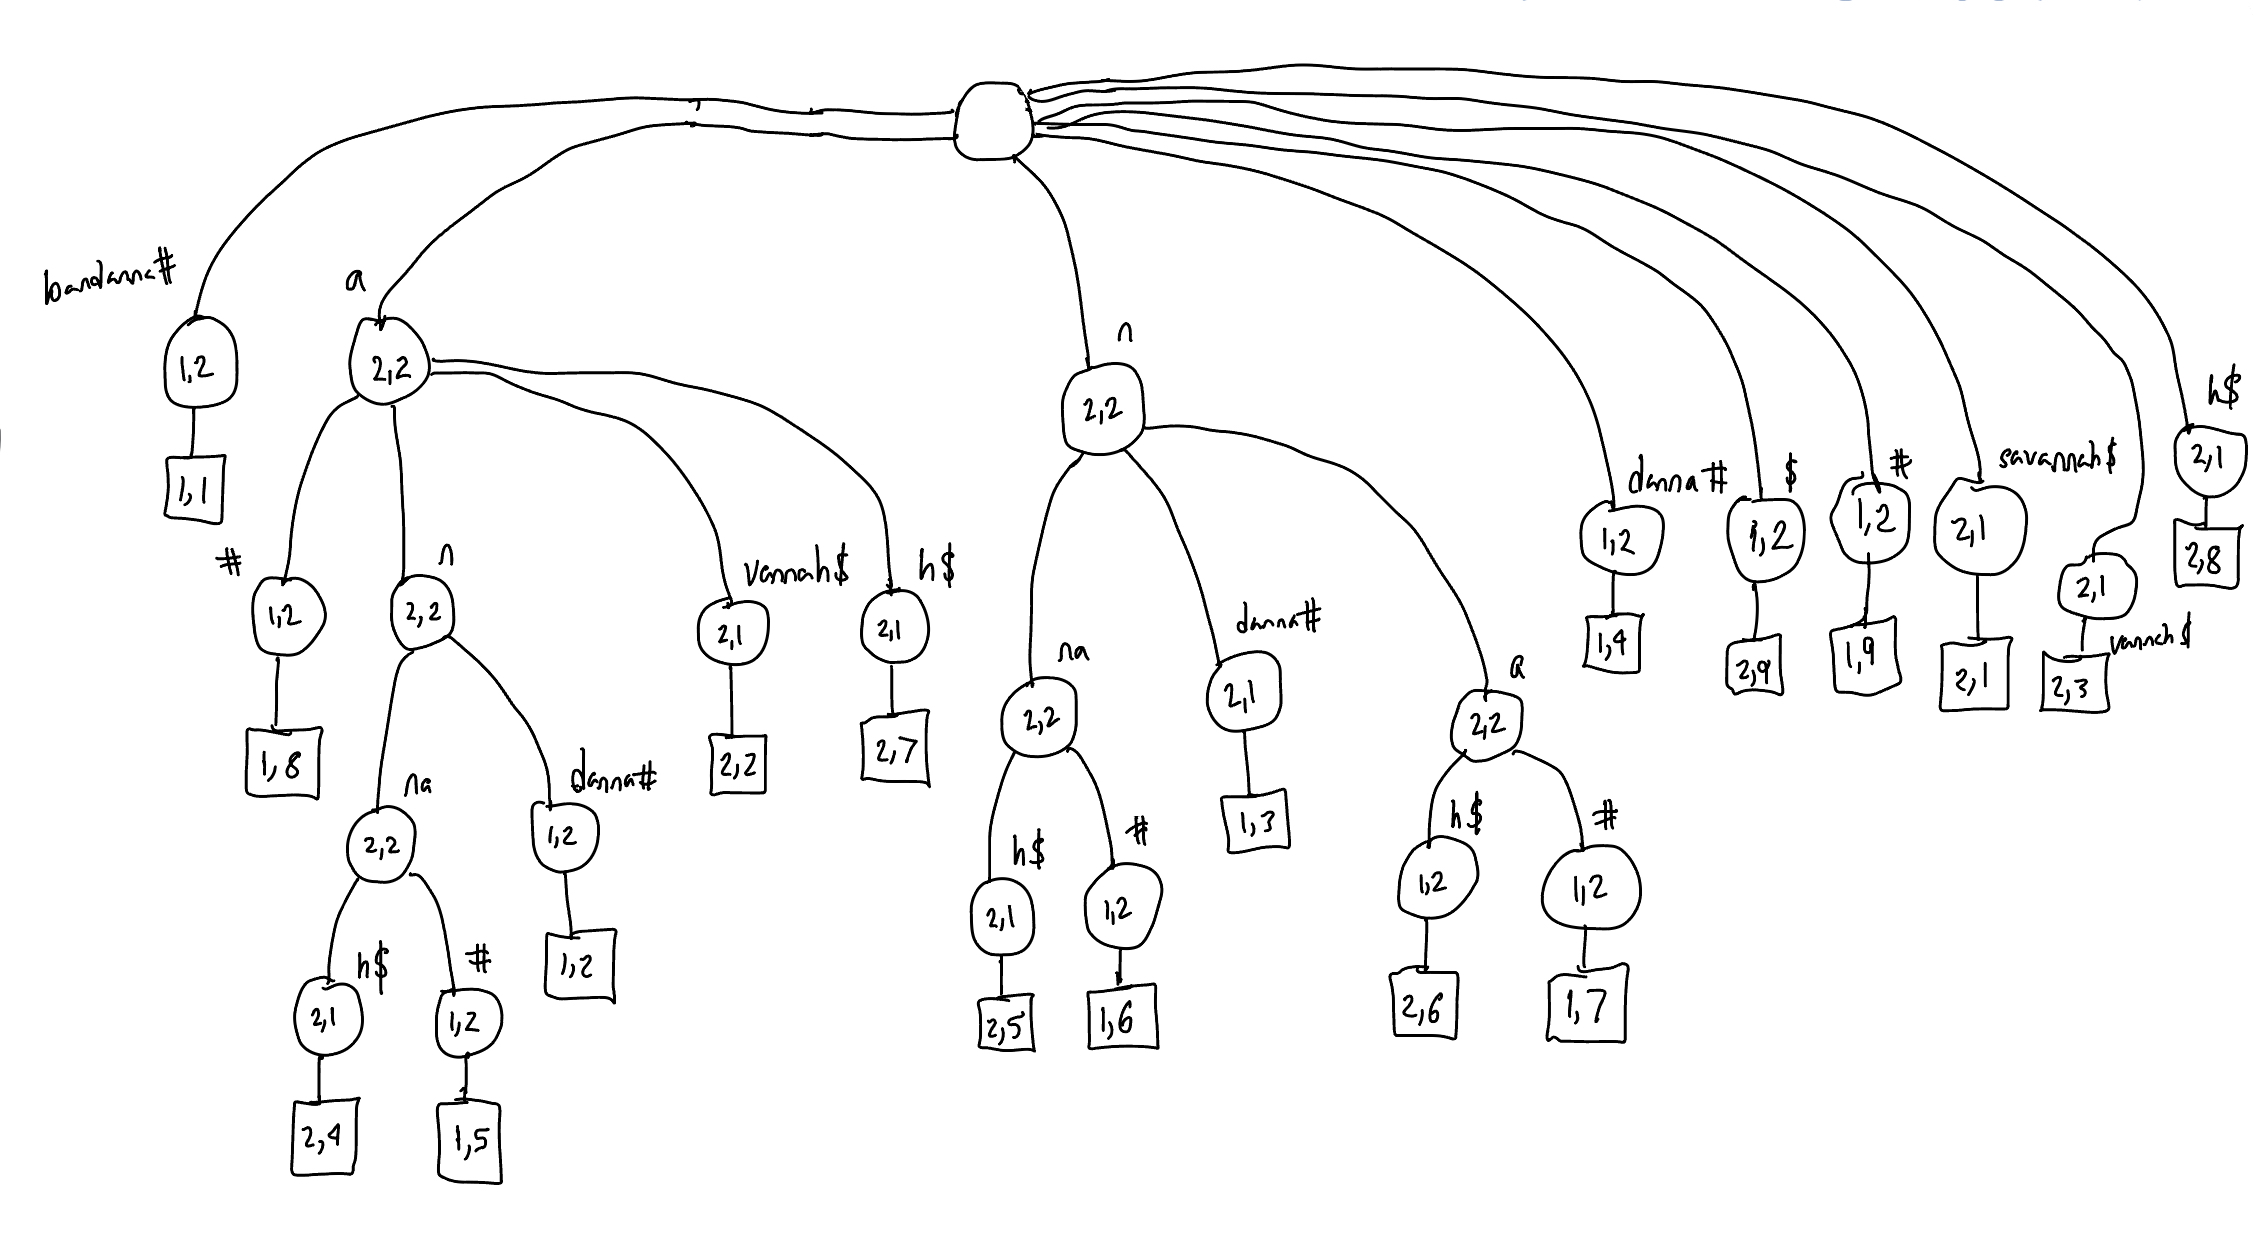
\includegraphics[width=0.8\textwidth]{suffix_tree.jpeg}
    \caption{Suffix Tree for BANDANNA\# and SAVANNAH\$}
    \label{fig:suffix_tree}
\end{figure}

\newpage
\subsection*{Part 2}

First, we must build a generalized suffix tree to contain the $m$ strings. Next, we must understand what the LCS of $m$ strings as represented by a suffix tree actually means. Since a suffix tree represents every suffix for the inserted strings, the LCS of $m$ strings would be represented by the path to the deepest internal node. This would correctly model the LCS of $m$ strings since the longest path to this node represents the longest common sequence shared by the given $m$ strings.

$\hfill \break$
Thus, we will utilize a depth-first-search in order to locate the path to the deepest internal node for the reasoning above. More specifically, we can start at the root node and traverse all possible paths of the suffix tree from the left to right. While going down the tree, we keep track of the number of edges required to hit a specific node, and update that number as we go along. Additionally, we also keep track of each node and how many edges are needed to hit it. We do this until we hit a leaf node, meaning the node has no further children. Once we hit a leaf node, we compare against the last longest path and update it if necessary, so that we know in the end which path is the longest.

$\hfill \break$
After recording the path, we can backtrack up one node and check if there are any additional paths to traverse, if there are, we repeat the same process to explore them all. If there are not, we go back up and repeat this process until we explore all paths in the tree. Once we have explored all paths, we can return the longest path we found.

\subsection*{Part 3}

The worst-case runtime of this algorithm is bounded under the sum of the number of suffixes for all of the strings. This can be represented as $O(m)$, where $m$ refers to $\sum_{i=0}^m \lvert S_i \rvert$, where the cardinality of $S_i$ refers to the string's number of suffixes. This is the case because we must traverse all possible paths in the suffix tree, and each path represents a suffix. Thus, the runtime is bounded by the number of suffixes for all of the strings.

\subsection*{Part 4}

In the case of BANDANNA\# and SAVANNAH\$, the longest common substring is ANNA, which can be seen as the deepest internal node in Figure 1.

\newpage
\section*{Problem 1 -- Reversible substrings (25\%)}    
    Let $S$ be a string of length $m$ and a \textit{substring} be a contiguous sequence of characters from $S$ identified by a tuple $S_{(i,l)}$ for starting index $i$ and length $l$.  
    Let the reverse of a string $S[0] S[1] \dots S[m-2] S[m-1]$ be $S[m-1]S[m-2] \dots S[1] S[0]$ denoted $S^-$.
    A \textit{reversible substring} is a substring  where $S_{(i,l)}=S^-_{(m-(i+l),l)}$. 
    Consider this example in Python:
    \begin{verbatim}
>>> S="PPABCDCBTTHMN"
>>> i=3
>>> l=5
>>> m=len(S)
>>>
>>> (S[::-1])[m-(i+l):m-(i+l)+l]
'BCDCB'
>>> S[i:(i+l)]
'BCDCB'
    \end{verbatim}
    Note that in the previous example we convert the length $l$ into an ending index for python.
    Intuitively, a reversible substring is a substring that is the same in the forward and reverse directions.

\begin{enumerate}
    \item Write an algorithm using suffix trees that computes the longest reversible substring of a string $S$. 
\textit{Hint: Think about using a suffix tree for multiple strings.}
    \item What is your algorithms runtime? Show your work/give an argument.
    \item Use your algorithm to find the longest reversible substring of the string RACECARS.
\end{enumerate}

\subsection*{Part 1}

Similarly to Question 0, we are able to utilize a suffix tree in order to find the LCS of the strings. However, in this case, we are looking for the longest reversible substring given a string $S$. In order to accomplish this, we can utilize a suffix tree and insert the strings $S$, and its reverse $S_r$. We will begin by creating a suffix tree containing these two strings.

$\hfill \break$
Now, with such a suffix tree created, we are able to utilize the same algorithm as Question 0, in which we utilize a depth-first-search to find the longest path to the deepest internal node. We are able to do this since the longest reversible substring for $S$ is nothing more than the longest common substring between $S$ and $S_r$. Thus, the deepest internal node in the suffix tree between $S$ and $S_r$ represents the longest reversible substring for $S$.

\subsection*{Part 2}

The algorithm's we devised above follows the same rules as the first problem, but with two strings. Since the two strings are the same, just reversed, the number of suffixes must be the same for $S$ and $S_r$. Thus, the runtime of this algorithm would be $O(n)$ since the algorithm is bounded under the amount of suffixes, which in this case is the same for both, leaving us with $2n$ suffixes, which is $O(n)$.

\subsection*{Part 3}

Using our algorithm, the longest reversible substring for RACECARS is RACECAR.

\newpage
\section*{Problem 2 -- Suffix Arrays (25\%)}
\begin{enumerate}
    \item Build the suffix array for string ``repetitive''.
    \item Recall the longest common prefix array, an array of size $m-1$ that stores the length of the longest common prefix for each pair of adjacent strings. 
Build the LCP array for ``repetitive''.
    \item Describe an algorithm for finding a substring pattern $P$ using suffix and LCP arrays.
    \item Consider this algorithm and the case where the alphabet is large, say, $O(m)$. Would you prefer to use suffix trees or suffix arrays? Why?
\end{enumerate}

\subsection*{Part 1 \& 2}

\begin{figure*}[!htb]
    \centering
    \begin{minipage}[t]{0.5\textwidth}
        \centering
        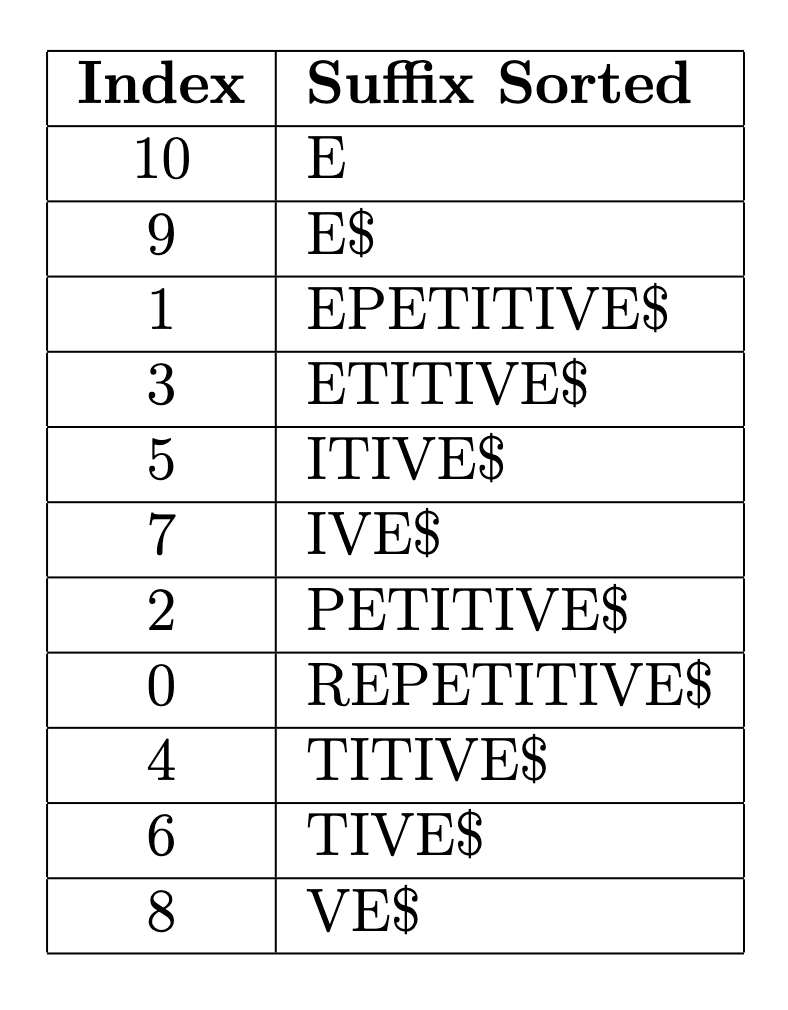
\includegraphics[width=0.8\textwidth]{suffix_array.png}
        \caption{Suffix Array for ``repetitive''}
        \label{fig:suffix_array}
    \end{minipage}%
    \begin{minipage}[t]{0.5\textwidth}
        \centering
        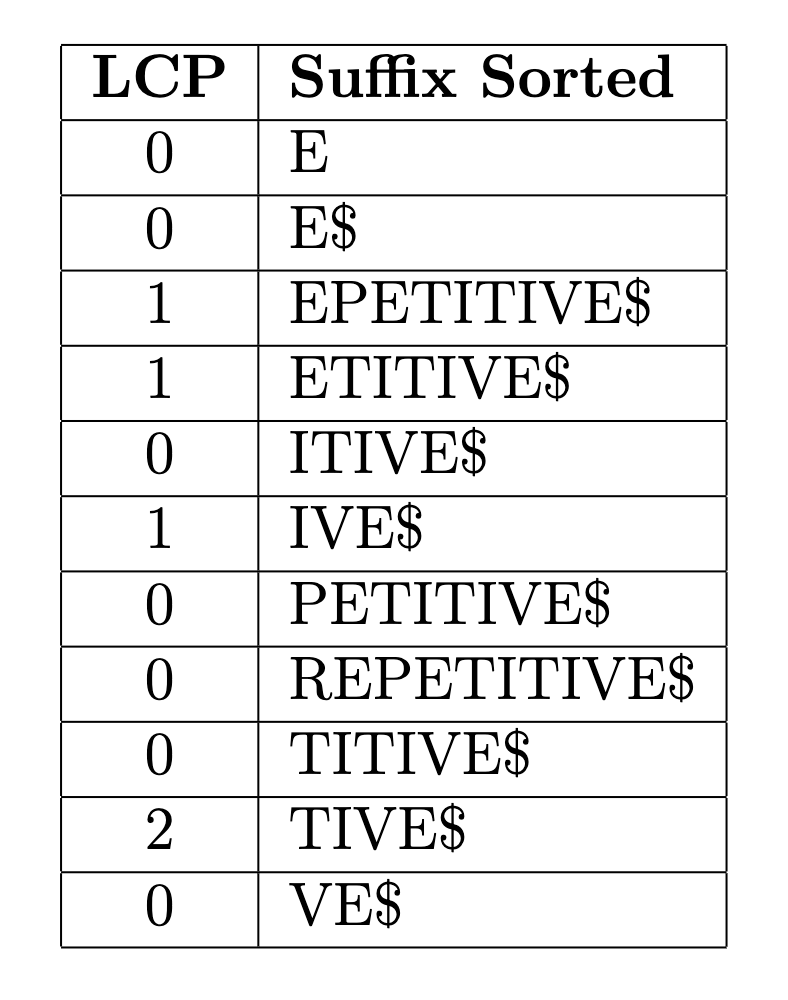
\includegraphics[width=0.8\textwidth]{lcp_array.png}
        \caption{LCP Array for ``repetitive''}
        \label{fig:lcp_array}
    \end{minipage}
\end{figure*}

\newpage
\subsection*{Part 3}

In order to find a substring pattern $P$ using suffix and LCP arrays, we can first construct the appropriate suffix and LCP arrays for a larger string $S$. Once we have the suffix and LCP arrays for $S$, we are able to utilize a binary search to determine the general range of indices for which $P$ can be found in $S$.

$\hfill \break$
By definition, an LCP array stores the length of longest common prefix for each pair of adjacent strings. Thus, we can utilize our LCP array for $S$ in order to determine the number of occurrences of $P$ in the larger string $S$. We can accomplish this by checking the LCP array's entries around the value we received from the binary search. From this, we can start at the index our binary search resulted in, and from here can move up and down to see if the LCP values are non-zero. If they are, this means that the value in the current index is the prefix of the next index's value. We can then repeat the process until we reach an LCP value that is less than the length of $P$. During this process, we will keep track of the number of occurrences by using a counter. This will give us the number of occurrences of $P$ in $S$. 

\subsection*{Part 4}

Suffix arrays would be preferable in a case where the alphabet is large. This is primarily due to the fact that suffix arrays are far easier to traverse due to them being sorted lexicographically and thus being able to utilize a binary search. This is in contrast to suffix trees, which are not sorted and thus would require a linear search in order to find the appropriate substring. Thus, in a case where the alphabet is large, we would prefer to use suffix arrays since they are far easier to traverse.

\newpage
\section*{Problem 3 -- Hashing (25\%)}
Consider the following simple hash function $h$ for mapping keys $z_j \in Z$ for $j=1,\dots ,n$ to array indices $\{1, \dots  m\}$.
For each key $z \in Z$, $h(z)=i$ with probability $1/m$ where $i=1, \dots , m$.
What is the expected number of keys such that $h(a)=h(b)$ over all keys $a \neq b$?
\textit{Hint: you want to define a similar random variable representing collisions as we did in Lecture 22 or Chapter 1.5 of the Algorithms textbook.}

$\hfill \break$
Let $X$ be a random variable that indicates the number of collisions between two keys $i$ and $j$ in the hash table. We can define $X$ as follows:

\begin{equation*}
    X = \begin{cases}
        1 & \text{if $i=j$} \\
        0 & \text{if $i \neq j$}
    \end{cases}
\end{equation*}

$\hfill \break$
Further, we are given the probability of the collision, $P(h(e_i) = h(e_j)) = \frac{1}{m}$. Based on this information, we can construct the following expression to model the collision event $X_{ij}$:

\begin{equation*}
    X = \sum_{i=1}^{n} \sum_{j=i+1}^{n} X_{ij}
\end{equation*}

$\hfill \break$
We can then compute the expectation of $X$ in order to determine the expected number of keys such that $h(a) = h(b)$ over all keys $a \neq b$.

\begin{equation*}
    E[X] = E\left[\sum_{i=1}^{n} \sum_{j=i+1}^{n} X_{ij}\right] \Rightarrow \sum_{i=1}^{n} \sum_{j=i+1}^{n} E\left[X_{ij}\right]
\end{equation*}

$\hfill \break$
However, we since already know the value of $E\left[X_{ij}\right] = \frac{1}{m}$, we can substitute it into the above equation and find the expected number of collisions:

\begin{align*}
    E[X] &= \sum_{i=1}^{n} \sum_{j=i+1}^{n} \frac{1}{m}\\\\
    &= \frac{n(n-1)}{2m}
\end{align*}

\end{document}